% !TEX root = ./main.tex
% !TEX encoding = UTF-8 Unicode
% !TEX program = pdflatex
% !TeX spellcheck = it_IT

\graphicspath{{Immagini/},{Immagini/prodotto_matrici/}}

\chapter{Prodotto Matrici}

\section{Traccia}
Confrontare in Java e in $C++$  l'esecuzione del prodotto di matrici quadrate
di dimensione: 10000, 100000, 1000000.\\
Il benchmark è utilizzato per valutare le prestazione dei
due linguaggi di programmazione.\\

\section{System Under Test}
La macchina target utilizzata per l'esecuzione degli algoritmi è:
\begin{itemize}
  \item \textbf{Processore}: Intel(R) Core(TM) i7-7700HQ @ 2.80GHz
  \item \textbf{Memoria Ram}: 16GB DDR4-2400MHz
  \item \textbf{Tipo sistema}: Windows 10 64bit, processore basato su x64
  \item \textbf{Storage}: SSD Kingston M.2.SATA 480GB
\end{itemize}

\section{Soluzione}
Il classico algoritmo di prodotto matriciale ha una complessità computazionale
$O(n^3)$, dunque l'esecuzione di tale algoritmo per le dimensioni assegnate
richiederebbe un tempo di esecuzione elevato.\\
Quindi si è scelto di ridurre notevolmente le dimensioni ed utilizzare l'algoritmo di
\textbf{Strassen} il quale ha una complessità computazionale $O(n^{2,81})$.\\

\subsection{Strassen Algorithm}
L'algoritmo di Strassen calcola il prodotto di matrici quadrate assumendo che siano
del tipo $2^n x 2^n$. \\ In particolare: $ C=A*B$ con $A,B,C \in R^{2^n x 2^n}$.\\
Dividendo le matrici A,B e C in blocchi si ottiene:
\\
\[
A =
\begin{bmatrix}
  A_{1,1} & A_{1,2} \\
  A_{2,1} & A_{2,2}
\end{bmatrix}
B =
\begin{bmatrix}
  B_{1,1} & B_{1,2} \\
  B_{2,1} & B_{2,2}
\end{bmatrix}
C =
\begin{bmatrix}
  C_{1,1} & C_{1,2} \\
  C_{2,1} & C_{2,2}
\end{bmatrix}
\]\\
con $A, B, C \in R^{2^{n-1} x 2^{n-1}}$.\\
\\
La matrice risultato si ottiene come:\\
$$C_{1,1} = A_{1,1}B_{1,1}+A_{1,2}B_{2,1}$$
$$C_{1,2} = A_{1,1}B_{1,2}+A_{1,2}B_{2,2}$$
$$C_{2,1} = A_{2,1}B_{1,1}+A_{2,2}B_{2,1}$$
$$C_{2,2} = A_{2,1}B_{1,2}+A_{2,2}B_{2,2}$$
\\
Utilizzando tale tecnica il numeri di prodotti da effettuare sono 8 , esiste
una tecnica che consente di effettuare un prodotto in meno.\\
Per utilizzare tale tecnica si definiscono le seguenti matrici:\\
$$M_1 = (A_{1,1}+A_{2,2})(B_{1,1}+B_{2,2})$$
$$M_2 = (A_{2,1}+A_{2,12})B_{1,1}$$
$$M_3 = A_{1,1}(B_{1,2}-B_{2,2})$$
$$M_4 = A_{2,2}(B_{2,1}-B_{1,1})$$
$$M_5 = (A_{1,1}+A_{1,2})B_{2,2}$$
$$M_6 = (A_{2,1}-A_{1,1})(B_{1,1}+B_{1,2})$$
$$M_7 = (A_{1,2}-A_{2,2})(B_{2,1}+B_{2,2})$$
Quindi la matrice risultato si ottime come:
$$C_{1,1} = M_1 + M_4 - M_5 + M_7$$
$$C_{1,2} = M_3 + M_5$$
$$C_{2,1} = M_2 + M_4$$
$$C_{2,2} = M_1 - M_2 + M_3 + M_6$$

\section{Analisi}

Gli algoritmi sono stati testati su matrici quadrate di dimensione 1024, 2048 e 4096.\\
Come analisi preliminare sono stati effettuate 15 osservazione per ogni dimensione,
per rendere le esecuzioni indipendenti gli algoritmi sono stati eseguiti tramite uno
script batch.\\
L'algoritmo è stato testato in Java anche disattivando il JIT(Just In Time)
compiler il quale ottimizza l'esecuzione dell'algoritmo.\\

\subsection{Numero di esperimenti}

Per determinare la dimensioni dei campioni si è fatto utilizzo della seguente formula:
$$n= {{100*z*s} \over{r*\overline{x}}}$$
Dove:
\begin{itemize}
  \item \textbf{\textit{z}}: $(1-{\alpha / 2})$-quantile della distribuzione normale
  per ottenere un intervallo di confidenza $100(1-\alpha)$;
  \item \textbf{\textit{s}}: deviazione standard del campione;
  \item \textbf{\textit{r}}: accuratezza percentuale;
  \item \textbf{\textit{$\overline{x}$}}: media del campione.
\end{itemize}

Nel caso in analisi $\alpha = 0.05$ ed $ r = 5\% $.

Nelle seguenti figure sono riportati i tempi raccolti negli esperimenti effettuati
e le relative statiche utilizzate per il calcolo di \textbf{n}.
\begin{figure}[!htbp]
  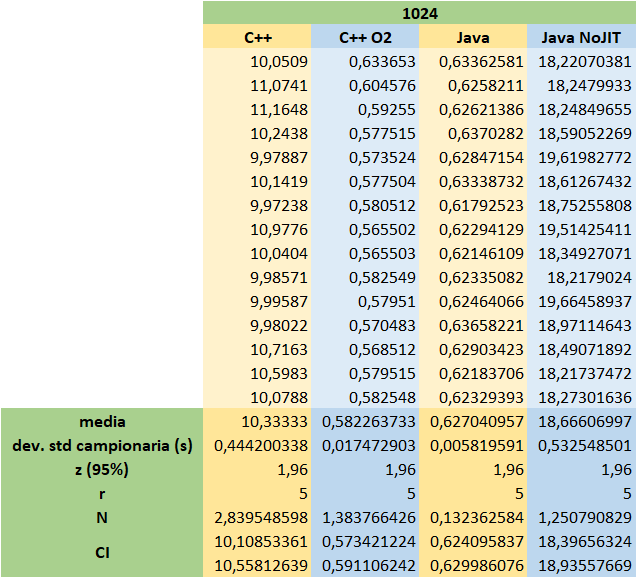
\includegraphics[width=1\linewidth,keepaspectratio]{tempi_1024}
  \caption{Esperimenti matrici 1024x1024}
  \label{tempi_1024}
\end{figure}

\begin{figure}[!htbp]
  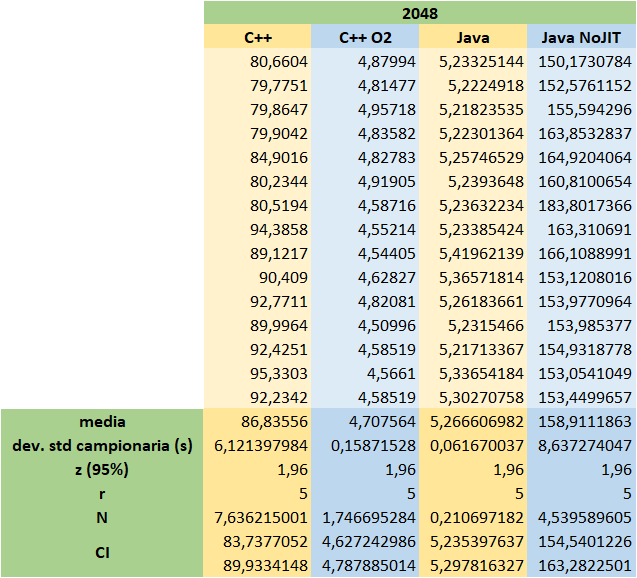
\includegraphics[width=1\linewidth,keepaspectratio]{tempi_2048}
  \caption{Esperimenti matrici 2048x2048}
  \label{tempi_2048}
\end{figure}

\begin{figure}[!htbp]
  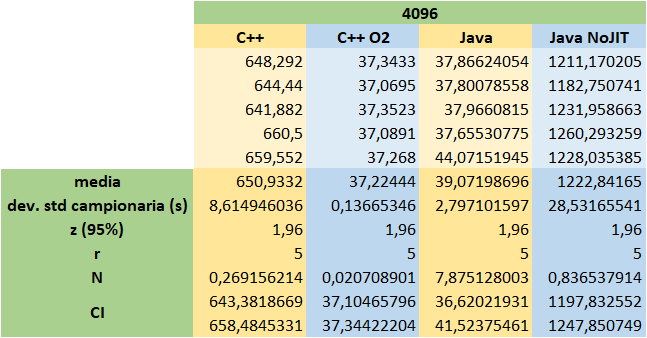
\includegraphics[width=1\linewidth,keepaspectratio]{tempi_4096}
  \caption{Esperimenti matrici 4096x4096}
  \label{tempi_4096}
\end{figure}

\clearpage

Considerando le tabelle riportate nell figure precedenti,
per la scelta del parametro \textbf{n} si considera il caso peggiore,
quindi il numero di esperimenti da effettuare è 8.\\

\subsection{Esperimenti}

Nelle figure sono riportate le tabelle contenenti i risultati per il confronto
dell'algoritmo di Strassen tra C++ e Java al crescere della dimensione. \\

\begin{figure}[!htbp]
  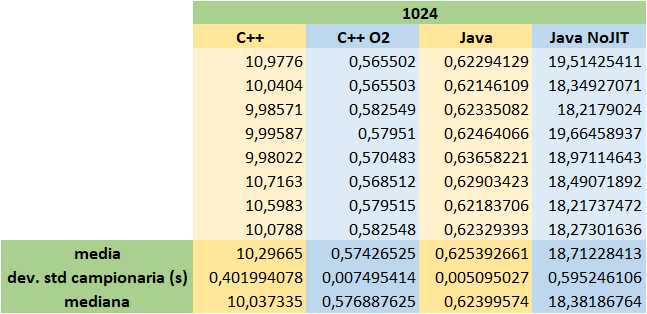
\includegraphics[width=1\linewidth,keepaspectratio]{tempi_8_1024}
  \caption{Esperimenti matrici 1024x1024}
  \label{tempi_8_1024}
\end{figure}

\begin{figure}[!htbp]
  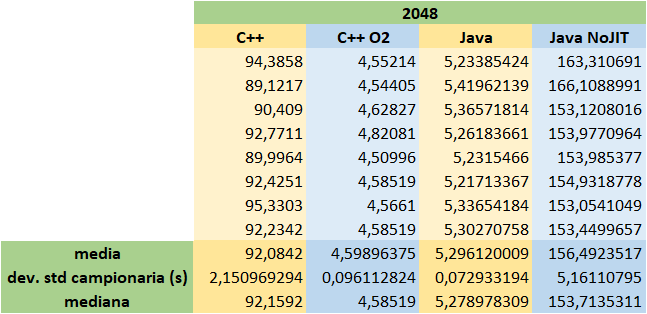
\includegraphics[width=1\linewidth,keepaspectratio]{tempi_8_2048}
  \caption{Esperimenti matrici 2048x2048}
  \label{tempi_8_2048}
\end{figure}

\begin{figure}[!htbp]
  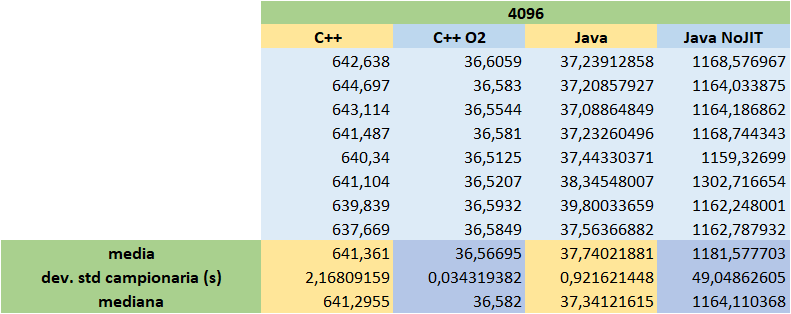
\includegraphics[width=1\linewidth,keepaspectratio]{tempi_8_4096}
  \caption{Esperimenti matrici 4096x4096}
  \label{tempi_8_4096}
\end{figure}

\clearpage

Nelle seguenti figure sono riportati i grafici ottenuti dalla tabelle degli esperimenti.\\

\begin{figure}[!htbp]
  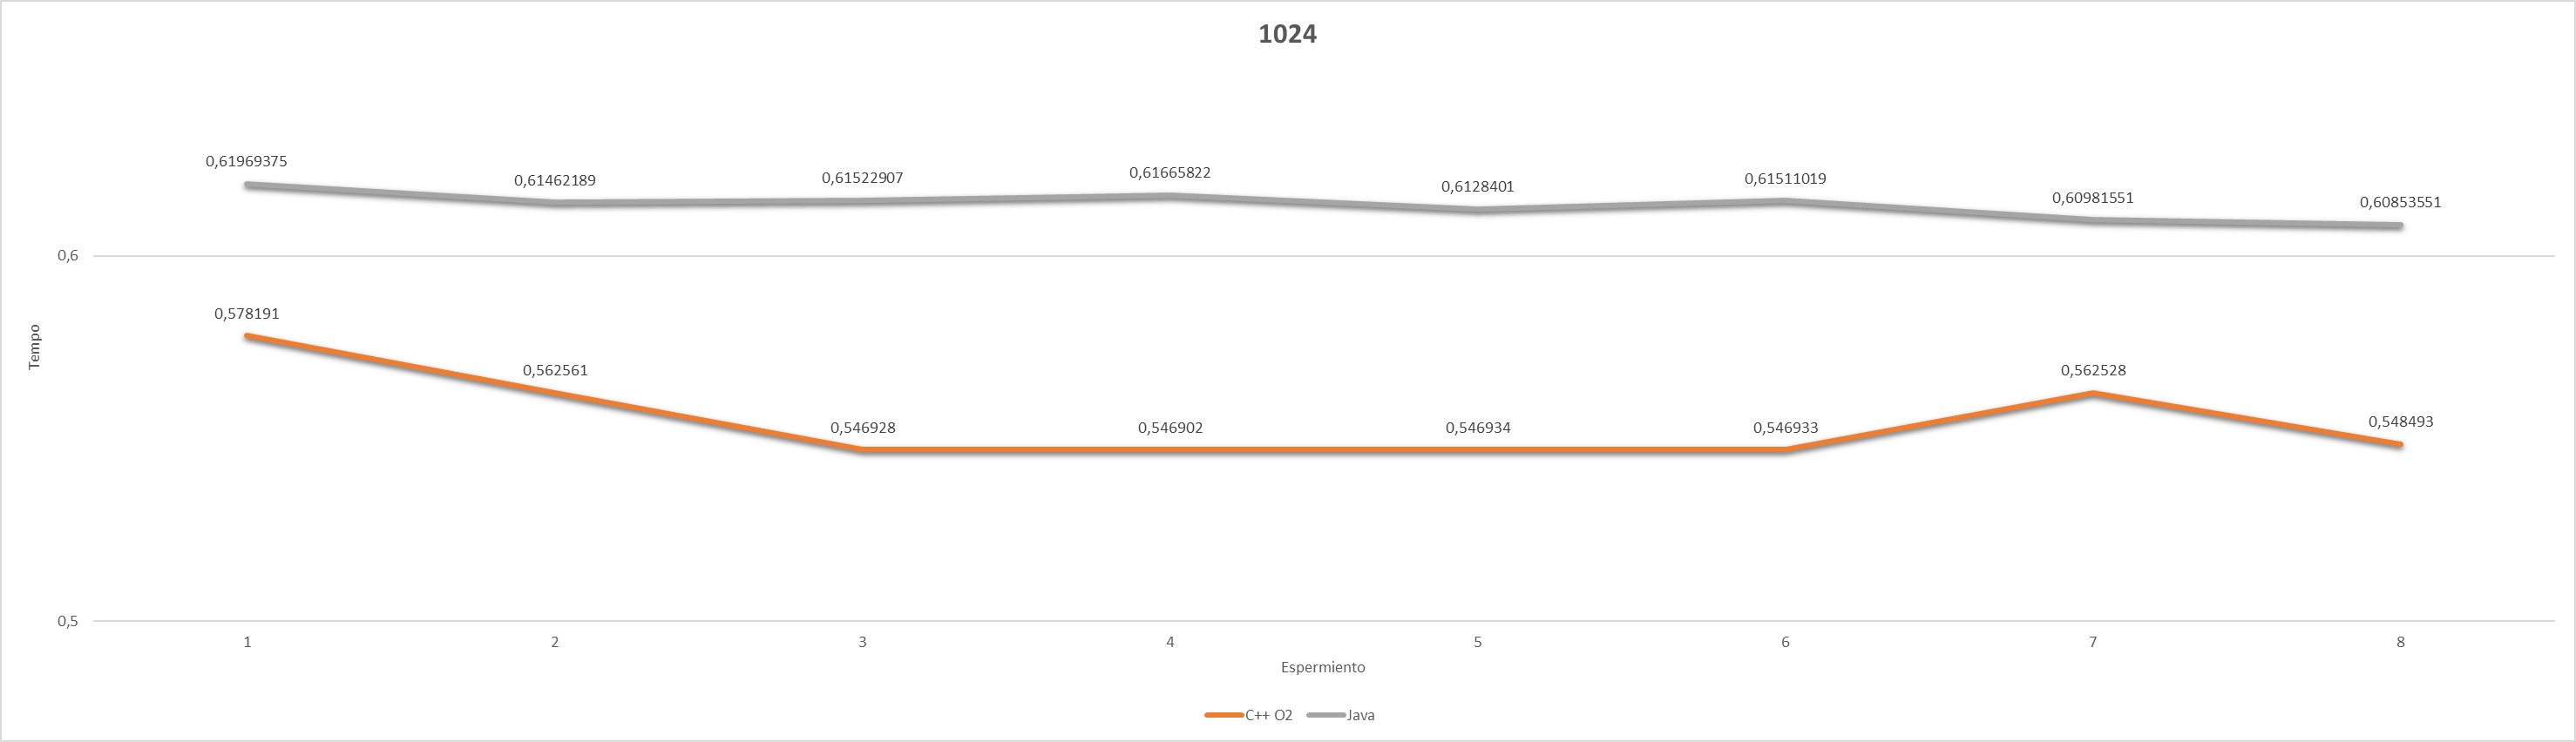
\includegraphics[width=1\linewidth,keepaspectratio]{grafico_tempi_1024_2}
  \caption{Confronto tempi Java C++ O2 1024x1024}
  \label{grafico_tempi_1024_2}
\end{figure}

\begin{figure}[!htbp]
  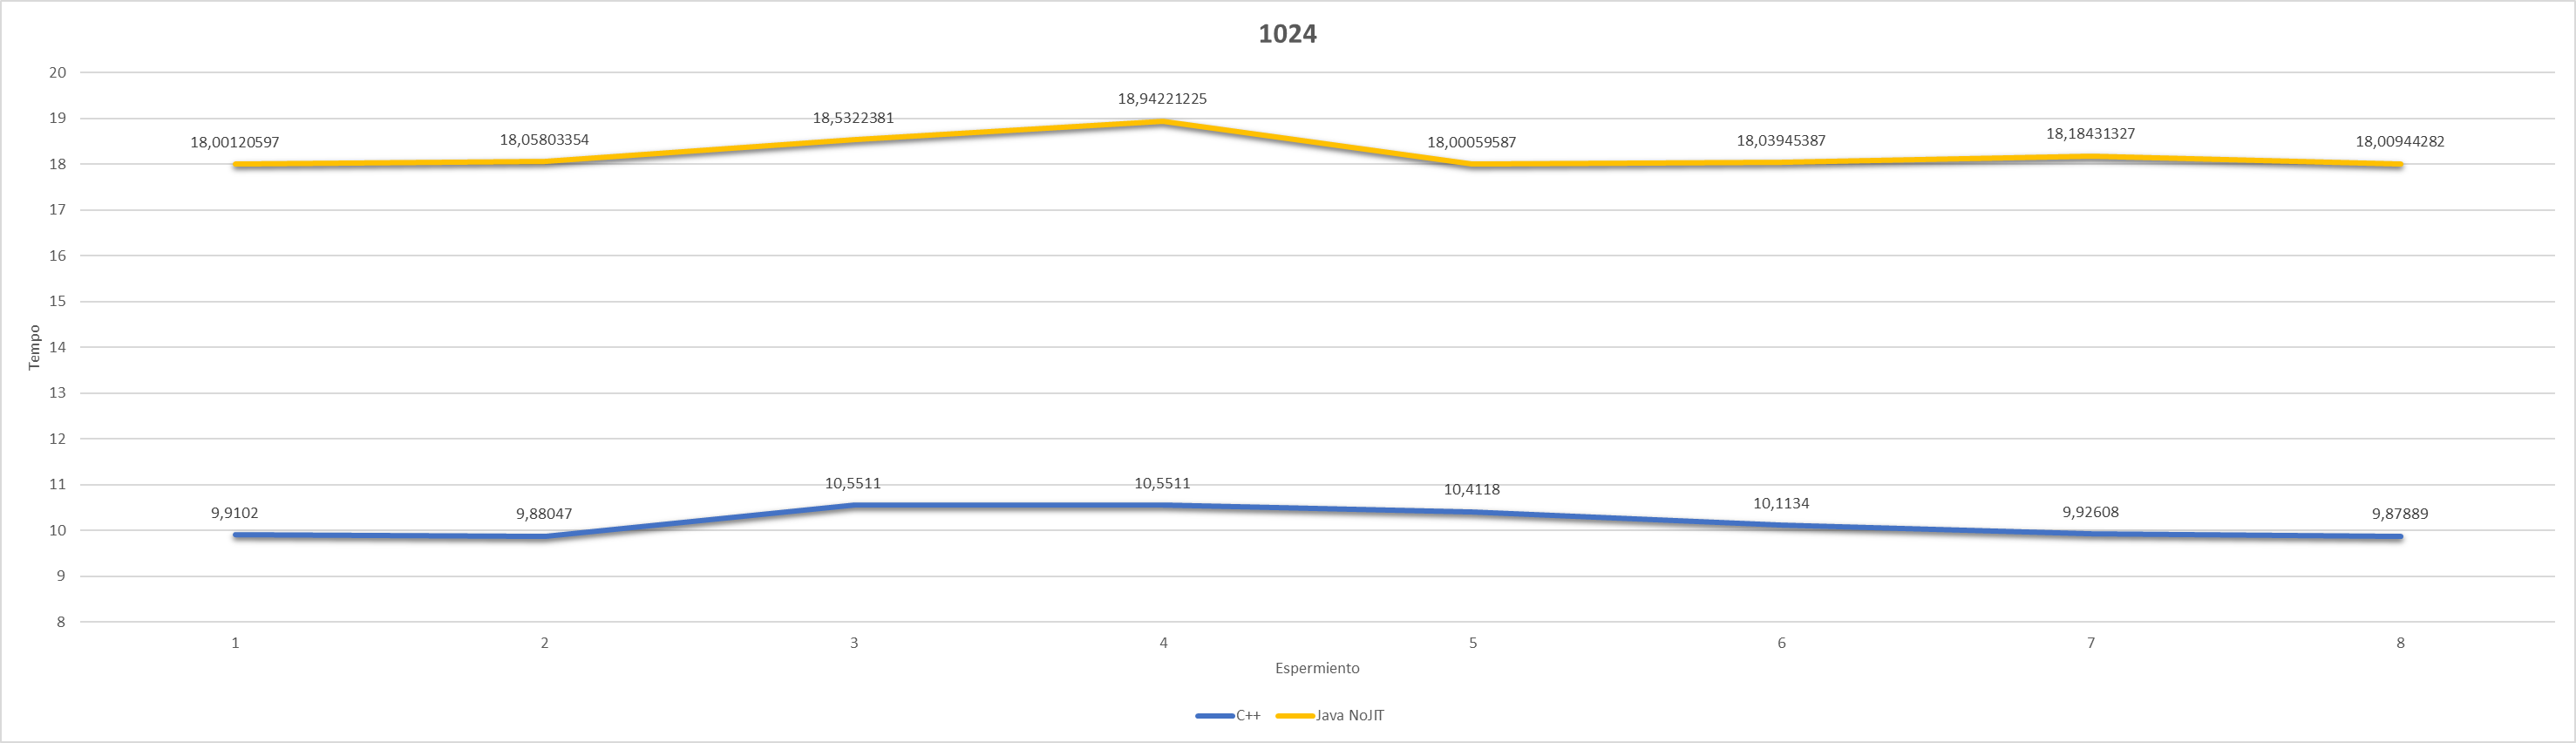
\includegraphics[width=1\linewidth,keepaspectratio]{grafico_tempi_1024_1}
  \caption{Confronto tempi Java con JIT disabilitato C++ 1024x1024}
  \label{grafico_tempi_1024_1}
\end{figure}

\begin{figure}[!htbp]
  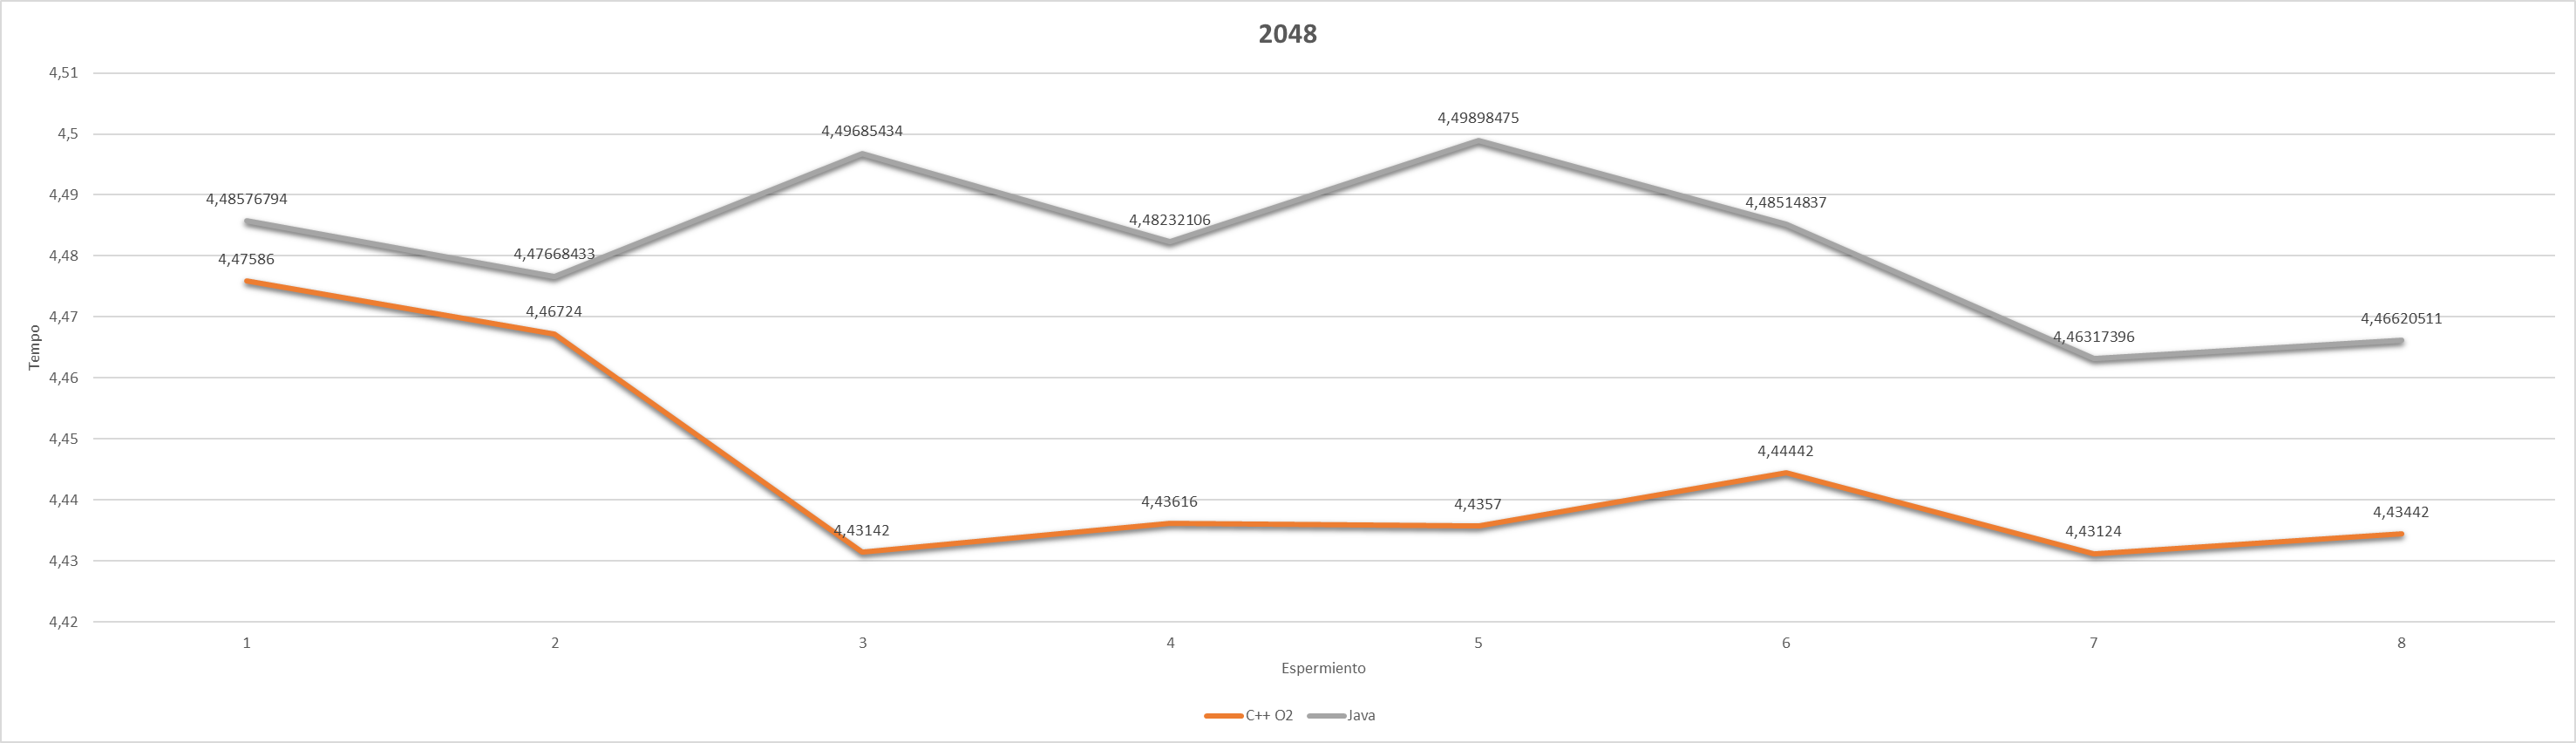
\includegraphics[width=1\linewidth,keepaspectratio]{grafico_tempi_2048_2}
  \caption{Confronto tempi Java C++ O2 2048x2048}
  \label{grafico_tempi_2048_2}
\end{figure}

\begin{figure}[!htbp]
  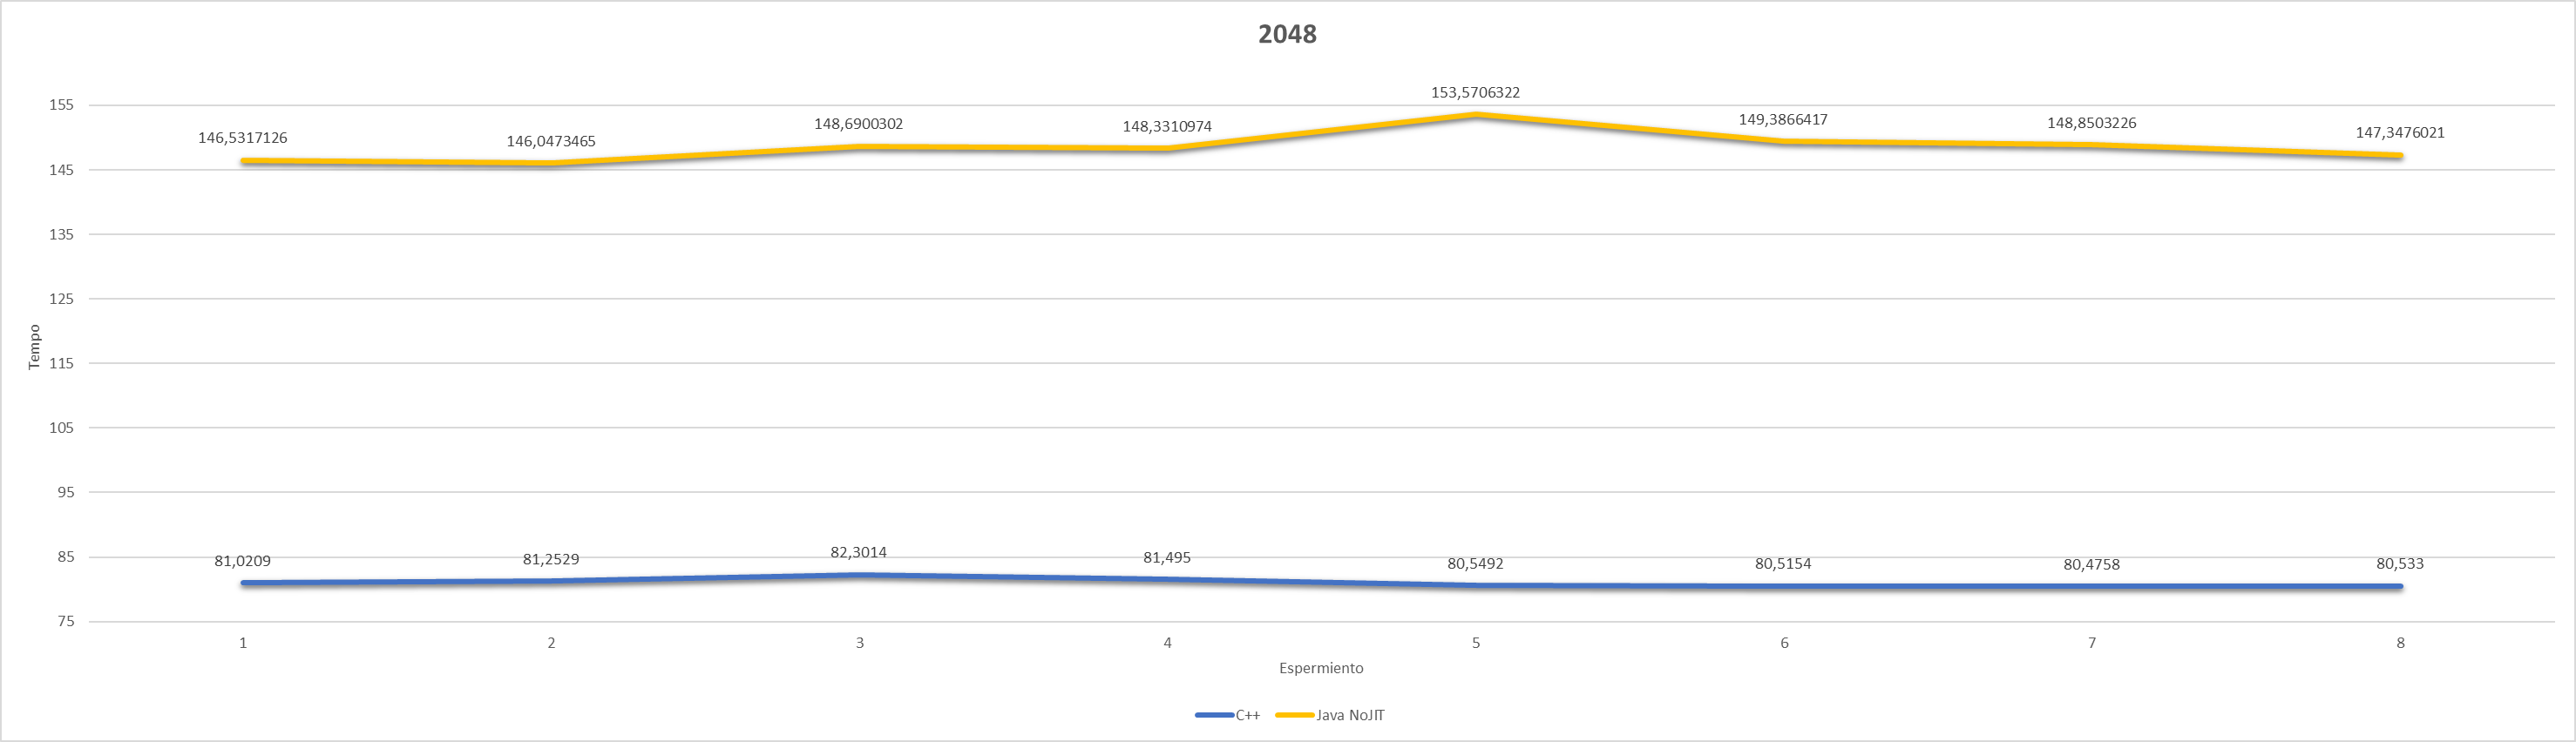
\includegraphics[width=1\linewidth,keepaspectratio]{grafico_tempi_2048_1}
  \caption{Confronto tempi Java con JIT disabilitato C++ 2048x2048}
  \label{grafico_tempi_2048_1}
\end{figure}

\begin{figure}[!htbp]
  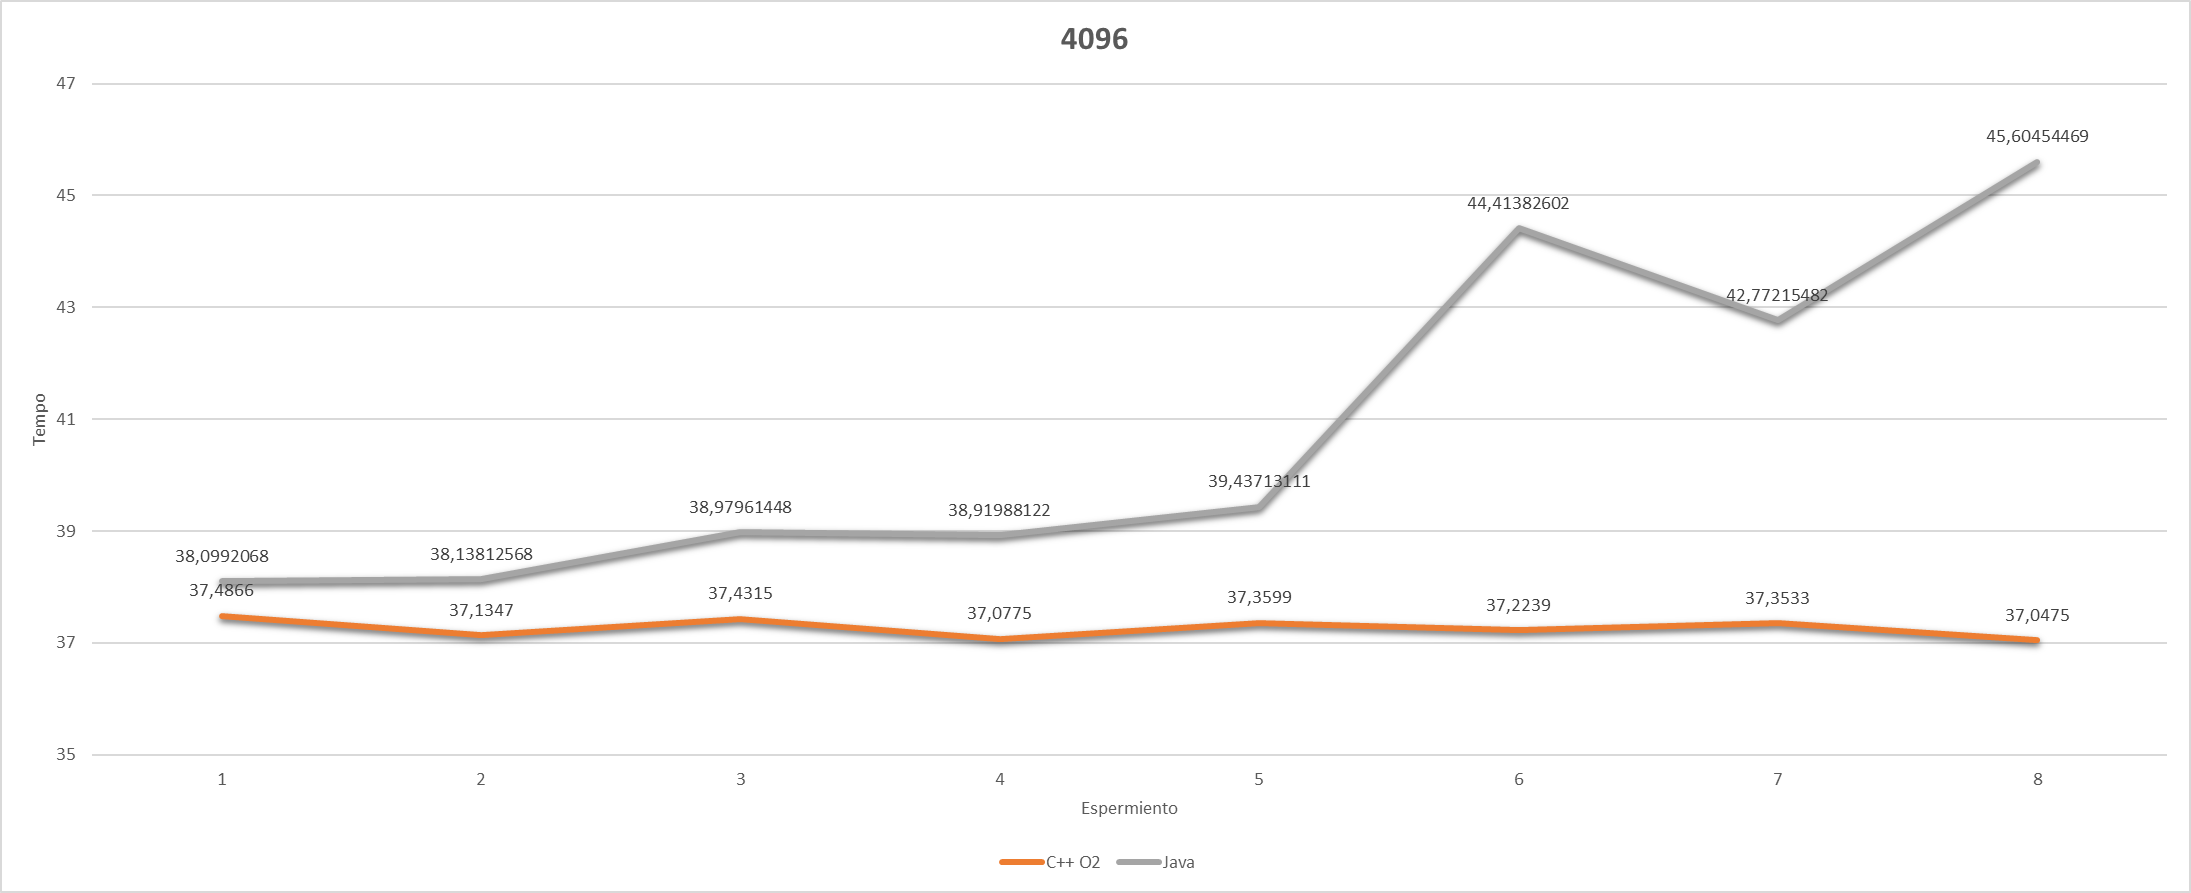
\includegraphics[width=1\linewidth,keepaspectratio]{grafico_tempi_4096_2}
  \caption{Confronto tempi Java C++ O2 4096x4096}
  \label{grafico_tempi_4096_2}
\end{figure}

\begin{figure}[!htbp]
  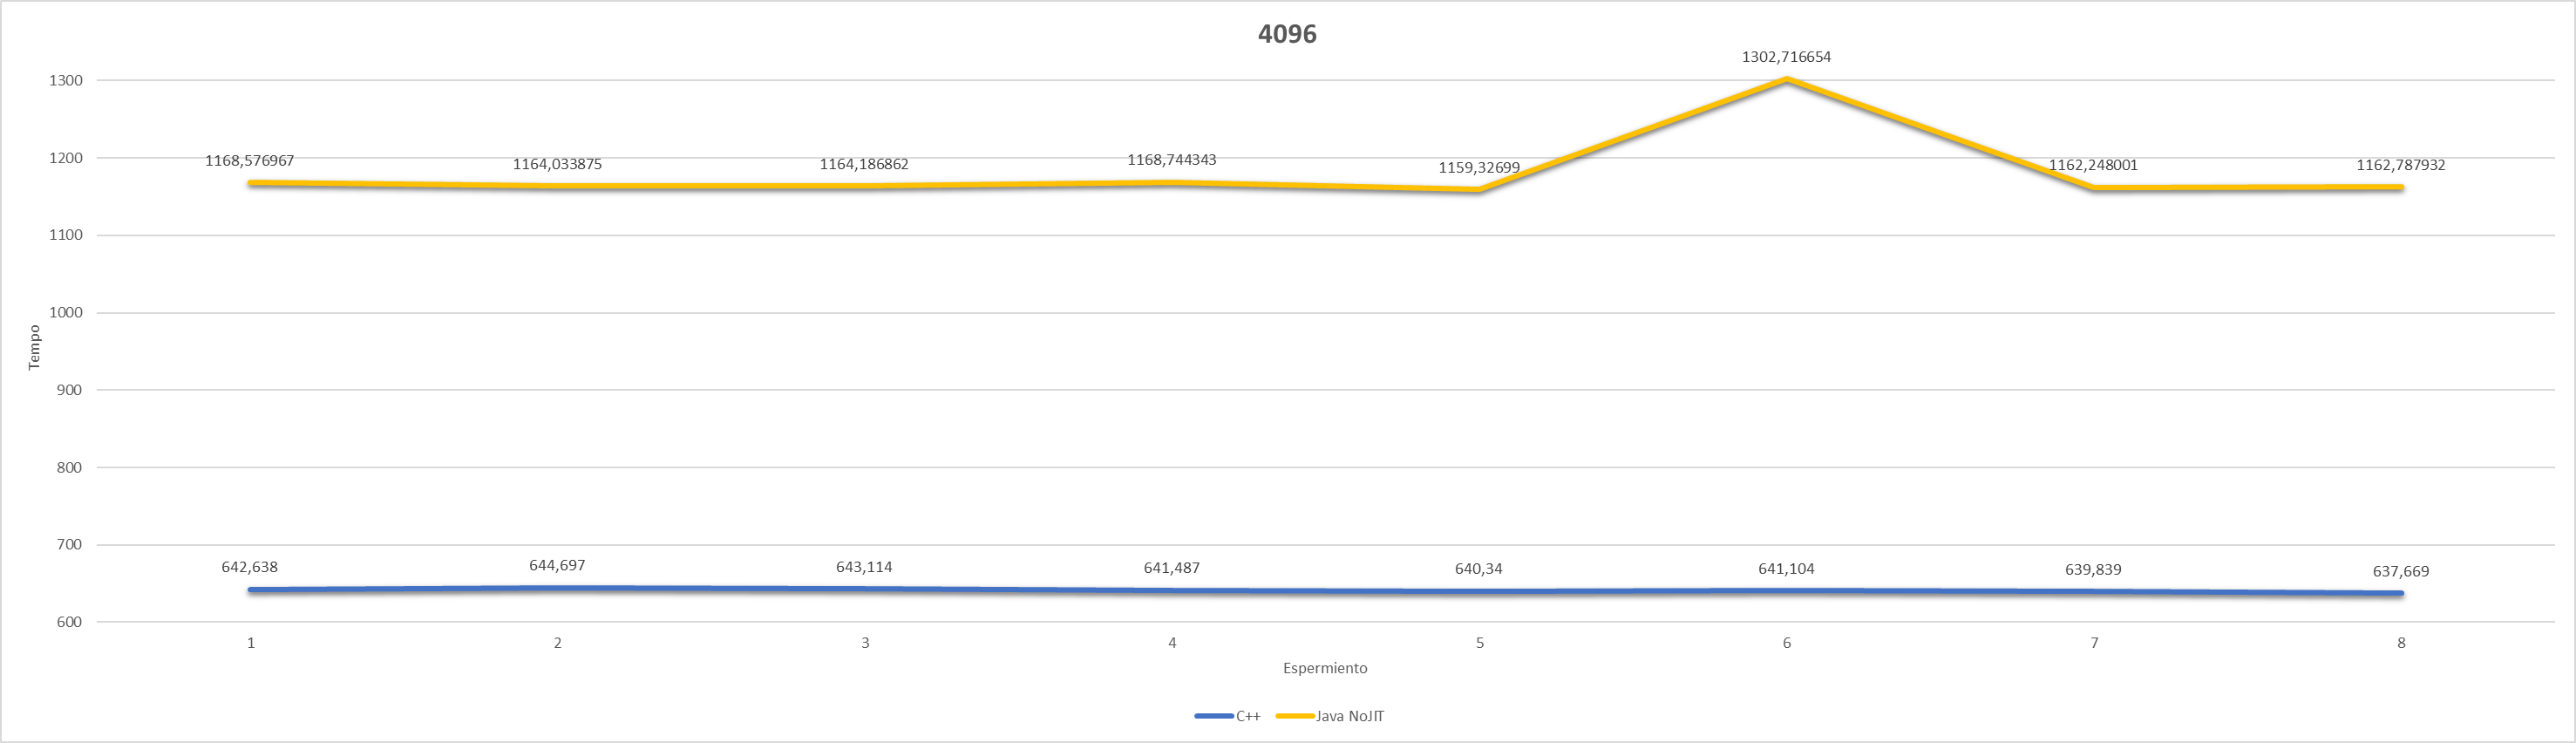
\includegraphics[width=1\linewidth,keepaspectratio]{grafico_tempi_4096_1}
  \caption{Confronto tempi Java con JIT disabilitato C++ 4096x4096}
  \label{grafico_tempi_4096_1}
\end{figure}

Come è possibile osservare per tutte le dimensioni considerate Java con JIT e C++ O2 son più veloci di C++ e
Java con JIT disattivato.\\

\subsection{Significatività dei risultati}

Per verificare la significatività statistica delle 8 osservazioni fatte è fondamentale
dimostrare che le distribuzioni non siano statisticamente equivalenti.\\
La statistica inferenziale mette a disposizione diversi test(parametrici e non),
i quali possono essere applicati in modo opportuno solo conoscendo il tipo di
distribuzione che si analizza.\\
Per individuare il tipo di distribuzione si fa utilizzo di alcuni parametri:

\begin{itemize}
  \item \textbf{Indice di Asimmetria}: cerca di fornire una misura sulla mancanza
  di simmetria in una distribuzione, il valore 0 è una condizione necessaria ma
  non sufficiente per la simmetria;
  \item \textbf{Curtosi}: fornisce una misura sull'appiattimento della curva,
  il valore dell'indice corrispondente ad una distribuzione normale è 0;
  \item \textbf{Coefficiente di Variazione}: permette di determinare la dispersione
  dei valori intorno alla media indipendentemente dall'unità di misura.
\end{itemize}
Si può utlizzare un test che verifica la normalità di una distribuzione che è il
test di Shapiro-Wilk o test della bontà di adattamento, tale test restituisce
il valore W che è compreso nell’intervallo [0, 1] dove valori di W vicini allo 0 indicano
una distribuzione skewed, mentre valori vicini a 1 indicano una distribuzione normale.
Un'altra tecnica per la verifica della normalità dei dati è di tipo visuale, osservando
il plot \textbf{Quantile-Quantile} se esso è approssimabile con una retta la distribuzione
è approsimabile con una normale, tale metodo è molto robusto agli errori.

\clearpage

\subsubsection{Distribuzioni C++ O2}
Nella seguente figura sono riportate le desctribuzioni al crescere di N per C++
con l'ottimizzazione O2 attiva.

\begin{figure}[!htbp]
  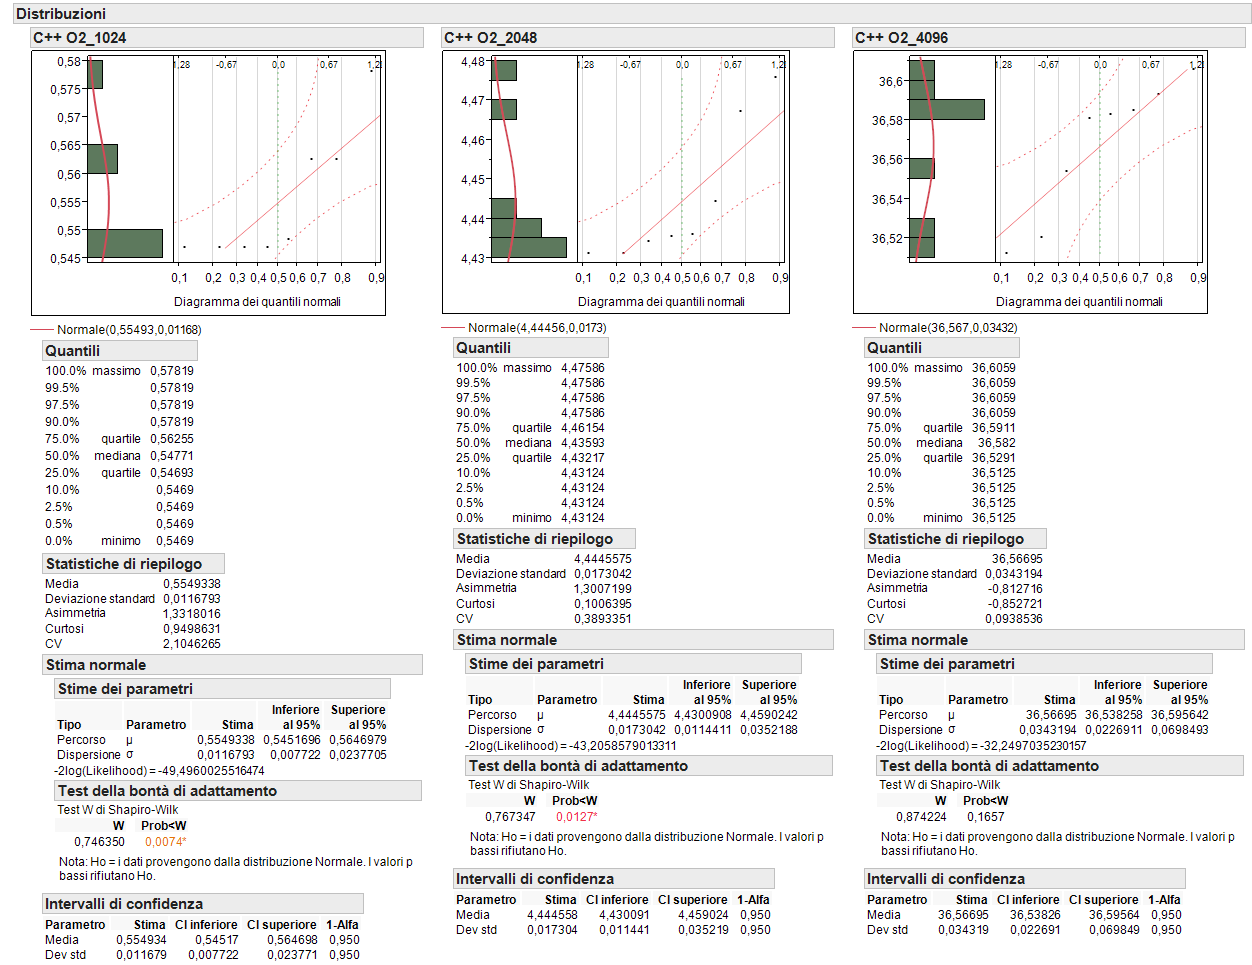
\includegraphics[width=1\linewidth,keepaspectratio]{distribuzione_cppO2}
  \caption{Distribuzioni osservazioni in C++ O2}
  \label{distribuzione_cppO2}
\end{figure}
Dalla \figurename~\ref{distribuzione_cppO2} si nota
che le distribuzioni per dimensione 1024 e 2048 non sono normali poichè è rifiutata
l'ipotesi nulla del test Shapiro-Wilk, mentre per la distribuzione a 4096 non è rigettata
l'ipotesi nulla quindi non possiamo affermare che non è normale ma possiamo avvalerci
di ulteriori parametri.\\
Osservando il plot Q-Q si osserva che la distribuzione non è approssimabile con una
retta e considerando anche gli indici di asimmetria e curtosi possiamo osservare che
la distribuzione è non normale.
\clearpage
\subsubsection{Distribuzioni C++ }
Nella seguente figura sono riportate le desctribuzioni al crescere di N per C++.

\begin{figure}[!htbp]
  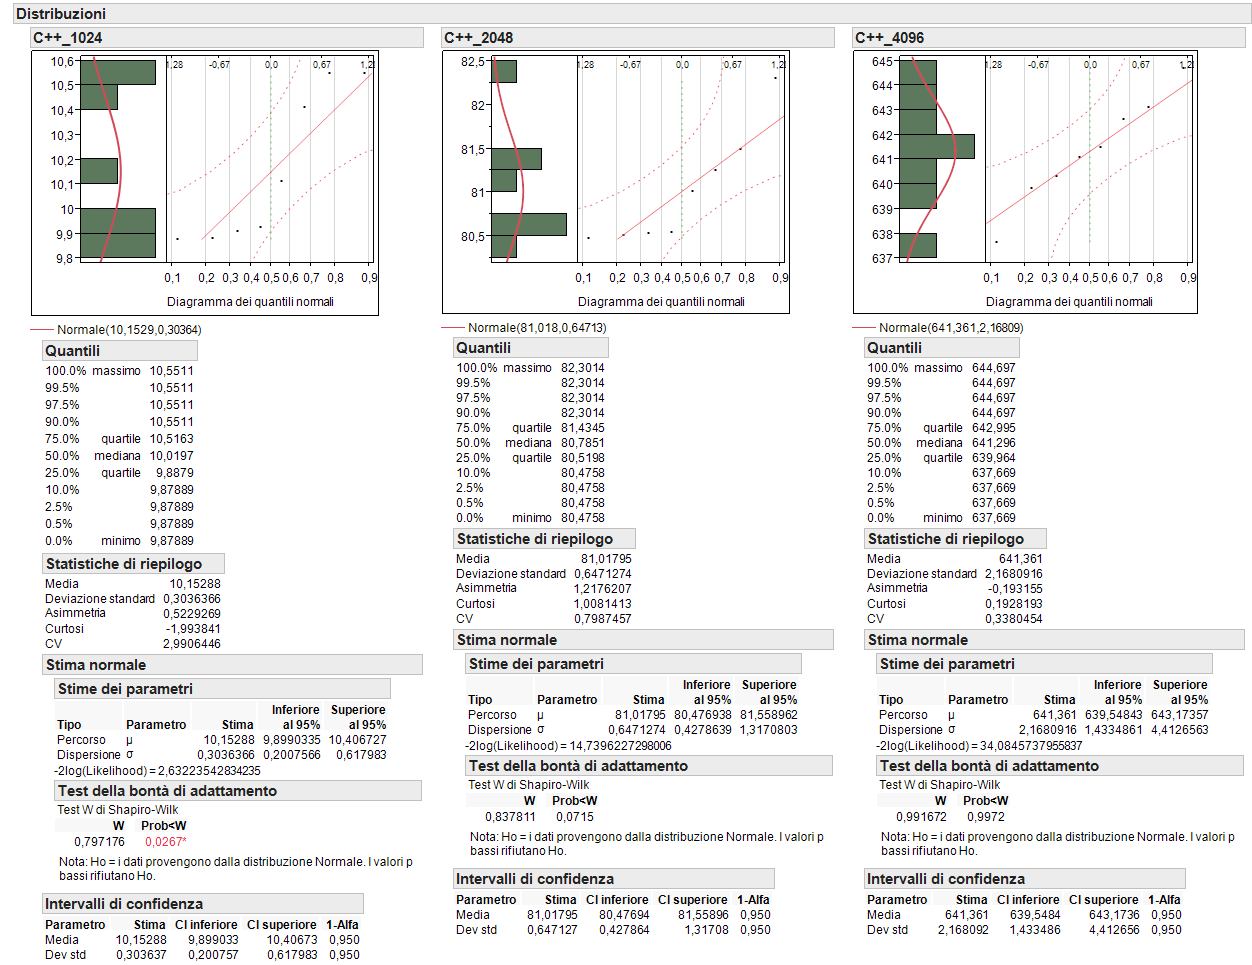
\includegraphics[width=1\linewidth,keepaspectratio]{distribuzione_cpp}
  \caption{Distribuzioni osservazioni in C++}
  \label{distribuzione_cpp}
\end{figure}

Dalla \figurename~\ref{distribuzione_cpp} si nota
che le distribuzioni per dimensione 1024 non è normale poichè è rifiutata
l'ipotesi nulla del test Shapiro-Wilk, mentre per la distribuzione a 2048 e 4096 non è rigettata
l'ipotesi nulla quindi non possiamo affermare che non sono normali ma possiamo avvalerci
di ulteriori parametri.\\
Osservando il plot Q-Q si osserva che la distribuzione con N pari a 2048 non è approssimabile con una
retta e considerando anche gli indici di asimmetria e curtosi possiamo osservare che
la distribuzione è non normale, mentre per la distribuzione 4096 dal plot Q-Q è approssimabile con una retta
e gli indici di asimmetria e curtosi ci indicano che è approssimabile con una normale.\\
\clearpage
\subsubsection{Distribuzioni Java}
Nella seguente figura sono riportate le desctribuzioni al crescere di N per Java.\\

\begin{figure}[!htbp]
  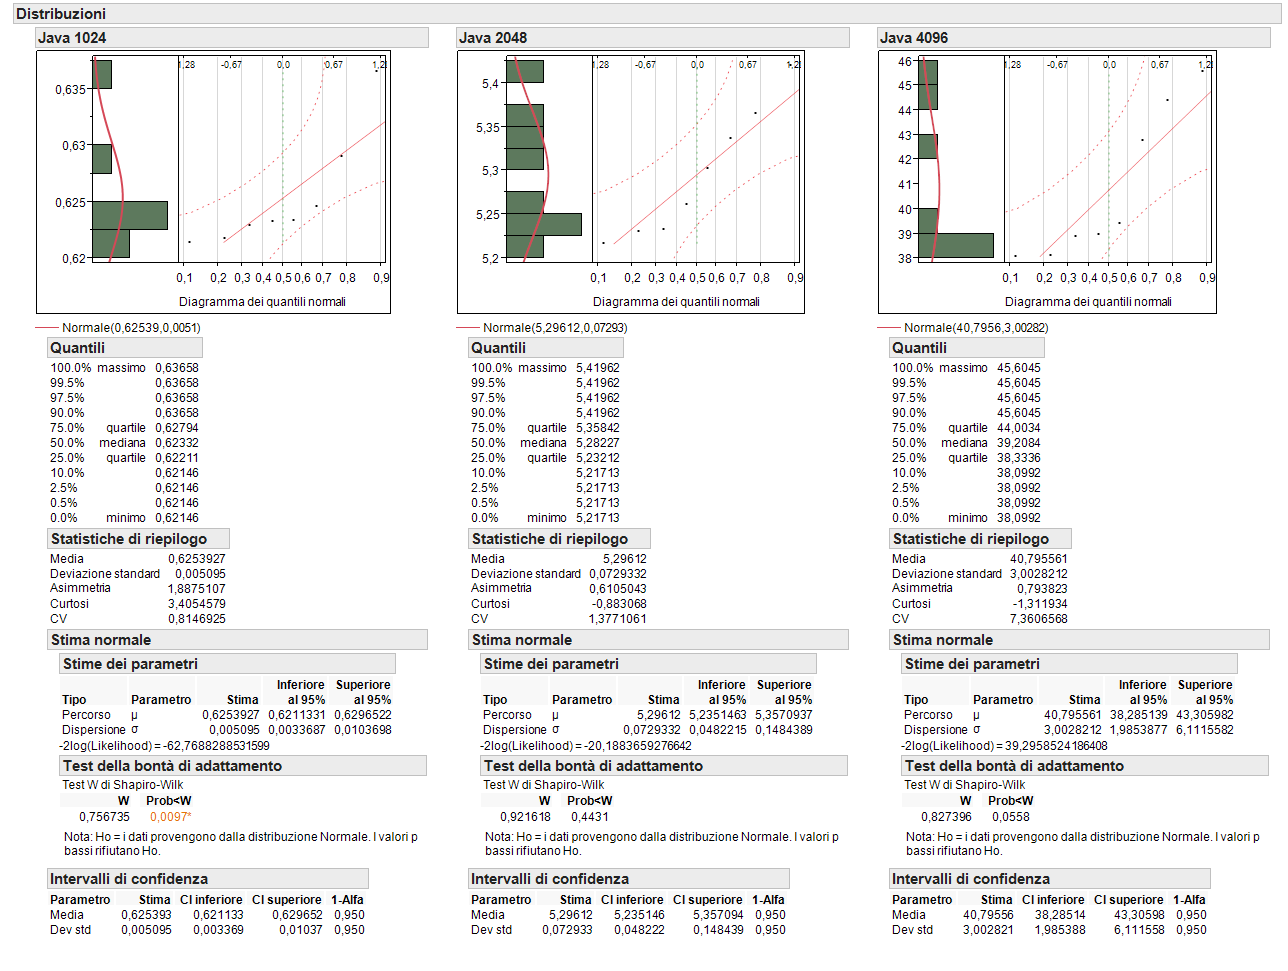
\includegraphics[width=1\linewidth,keepaspectratio]{distribuzione_java}
  \caption{Distribuzioni osservazioni in Java}
  \label{distribuzione_java}
\end{figure}

Dalla \figurename~\ref{distribuzione_java} si nota
che le distribuzioni per dimensione 4096 non è normale poichè è rifiutata
l'ipotesi nulla del test Shapiro-Wilk, mentre per le distribuzioni a 1024 e 2048 non è rigettata
l'ipotesi nulla quindi non possiamo affermare che non sono normali ma possiamo avvalerci
di ulteriori parametri.\\
Osservando il plot Q-Q si osserva che entrambe la distribuzione con N pari a 1024
si può approssimare con una retta e considerando anche gli indici di asimmetria e curtosi possiamo osservare che
le distribuzioni può essere considerata normale, mentre per N pari a 2048 non è verificata la normalità.\\
\clearpage
\subsubsection{Distribuzioni Java No JIT}
Nella seguente figura sono riportate le desctribuzioni al crescere di N per Java.\\

\begin{figure}[!htbp]
  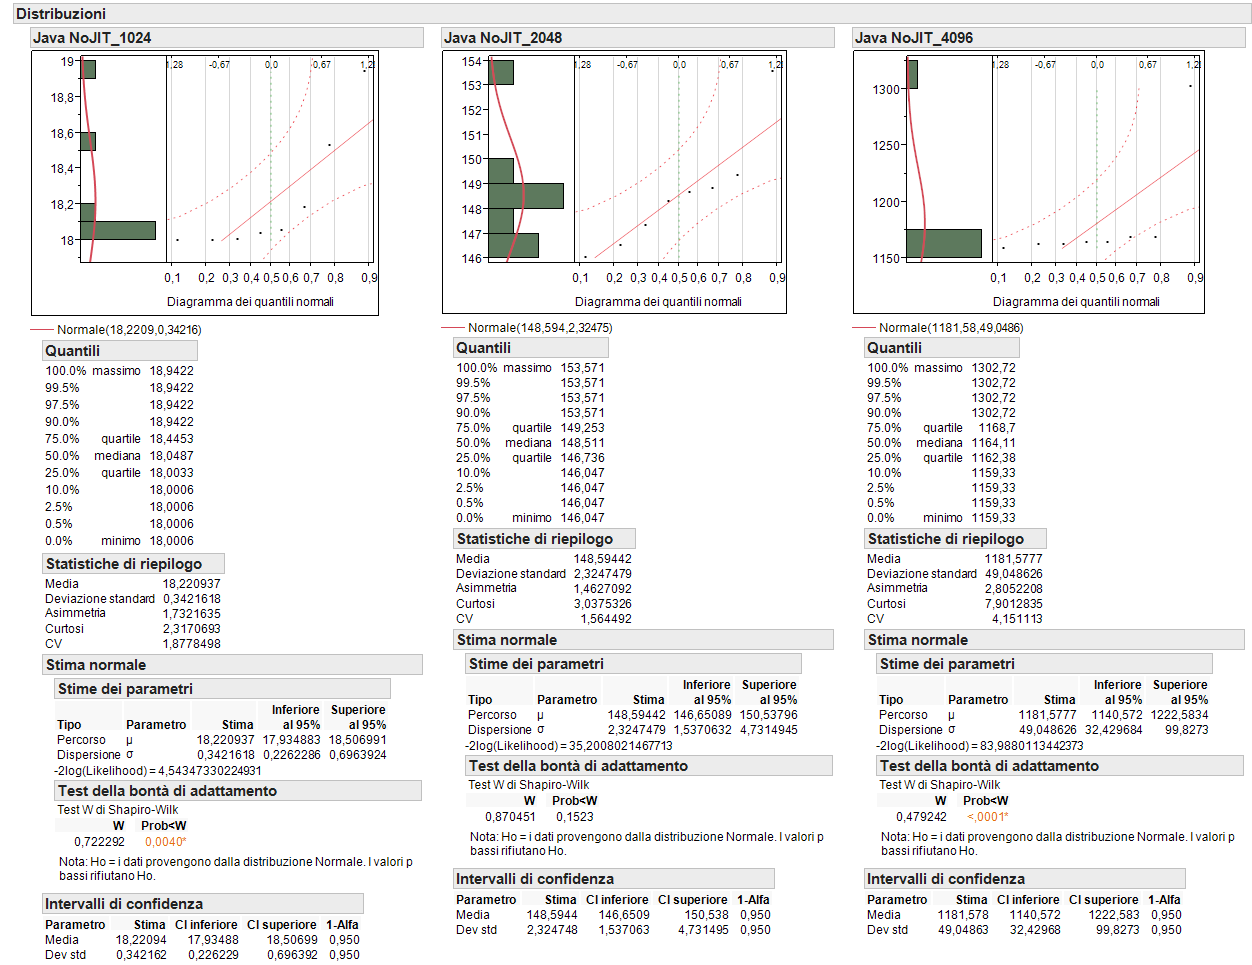
\includegraphics[width=1\linewidth,keepaspectratio]{distribuzione_javaNoJIT}
  \caption{Distribuzioni osservazioni in Java}
  \label{distribuzione_javaNoJIT}
\end{figure}

Dalla \figurename~\ref{distribuzione_javaNoJIT} si nota
che le distribuzioni per dimensione con n pari a 1024 e 4096 non sono normali poichè è rifiutata
l'ipotesi nulla del test Shapiro-Wilk, mentre per la distribuzione a 2048 non è rigettata
l'ipotesi nulla quindi non possiamo affermare che non sono normali ma possiamo avvalerci
di ulteriori parametri.\\
Osservando il plot Q-Q si osserva che entrambe la distribuzione con N pari a 2048
si potrebbe approssimare con una retta ma considerando  gli indici di asimmetria e curtosi possiamo osservare che
le distribuzioni non può essere considerata normale poichè sono molto maggiori di 0.
\clearpage
\subsubsection{Intervallo di confidenza}
Un’ultima osservazione da dover fare riguarda gli intervalli di confidenza ottenuti in
analisi preliminare.\\
Se si confrontano le mediane delle distribuzioni dei campioni
con gli intervalli di confidenza ottenuti in analisi preliminare si nota che non
tutte le distribuzioni rispettano le ipotesi fatte. Questo significa che l’ipotesi
di normalità fatta in analisi preliminare per alcune delle distribuzioni potrebbe venir meno.\\
Di seguito è riportata una tabella che riassume gli intervalli di confidenza
ottenuti in analisi preliminare e le medie ottenute dai campioni raccolti successivamente.

\begin{figure}[!htbp]
  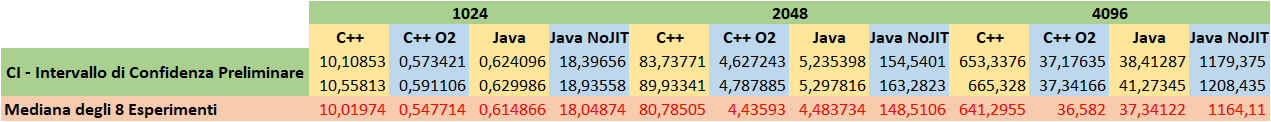
\includegraphics[width=1\linewidth,keepaspectratio]{CI_mediana}
  \caption{Intervalli di confidenza}
  \label{CI_mediana}
\end{figure}
\clearpage
\subsection{Validazione campioni}
Per le considerazioni fatte si deciso di caratterizzare il workload con la Mediana,
poichè solo 2 distribuzioni possono essere considerate normali.\\
Per verificare la significatività dei campioni non è più possibile applicare il test T-Test,
ma bisogna affidarsi a test non parametrici come il test di Wilcoxon/Kruskal-Wallis.\\
Il test di Kruskal-Wallis serve a verificare se più campioni indipendenti appartengono alla
stessa popolazione.\\
Di seguito vengono mostrati i risultati ottenuti da JMP.\\

\begin{figure}[!htbp]
  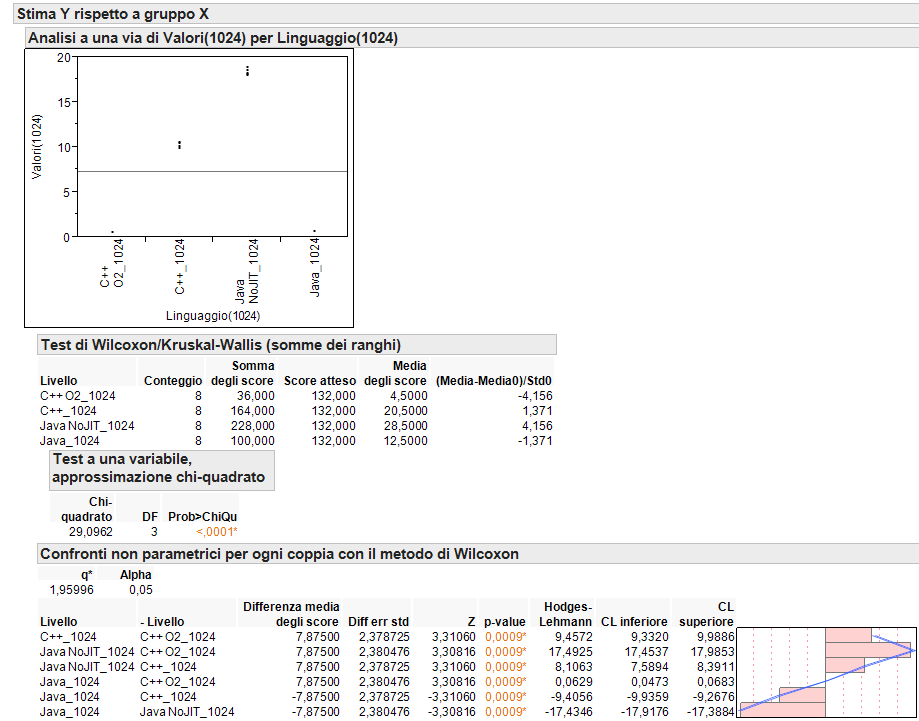
\includegraphics[width=1\linewidth,keepaspectratio]{Wilcoxon_Kruscal-Wallis_1024}
  \caption{Test di Wilcoxon/Kruscal-Wallis con matrici quadrate di dimensione 1024}
  \label{Wilcoxon_Kruscal-Wallis_1024}
\end{figure}

\begin{figure}[!htbp]
  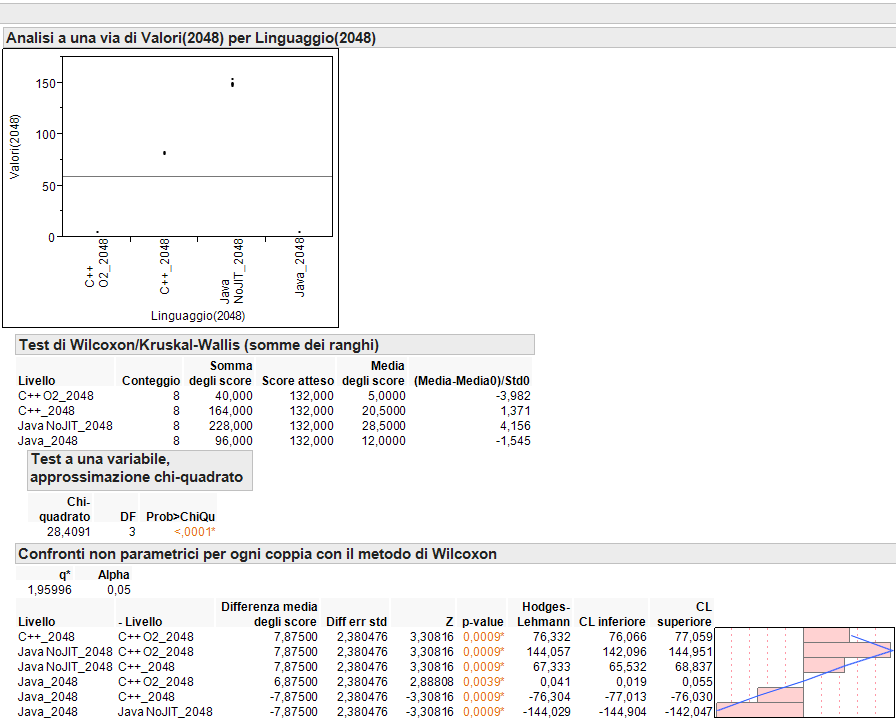
\includegraphics[width=1\linewidth,keepaspectratio]{Wilcoxon_Kruscal-Wallis_2048}
  \caption{Test di Wilcoxon/Kruscal-Wallis con matrici quadrate di dimensione 2048}
  \label{Wilcoxon_Kruscal-Wallis_2048}
\end{figure}

\begin{figure}[!htbp]
  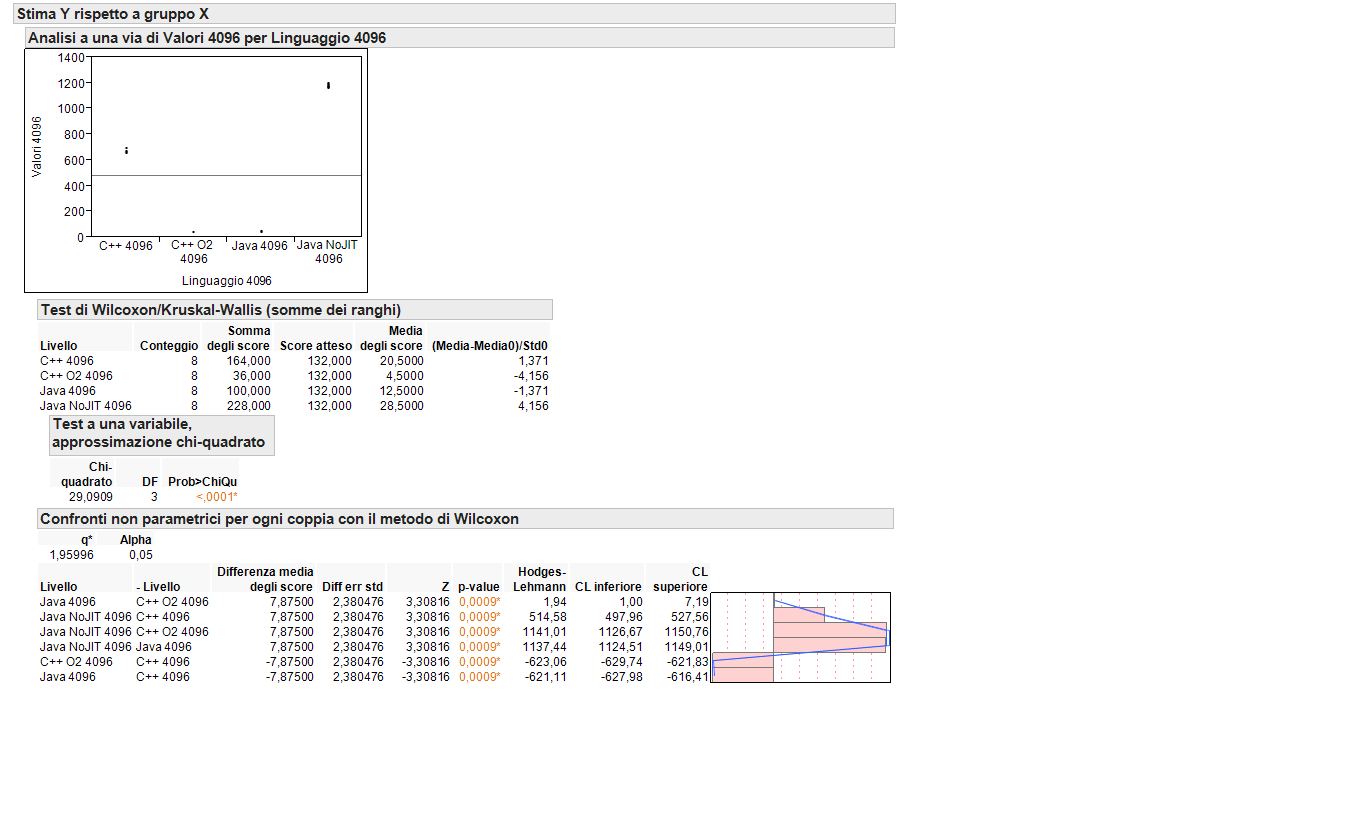
\includegraphics[width=1\linewidth,keepaspectratio]{Wilcoxon_Kruscal-Wallis_4096}
  \caption{Test di Wilcoxon/Kruscal-Wallis con matrici quadrate di dimensione 4096}
  \label{Wilcoxon_Kruscal-Wallis_4096}
\end{figure}

Dal test effettuato si può concludere affermando che i campioni probabilmente
provengano da popolazioni differenti.

\clearpage

\section{Conclusioni}
Concludendo se si fa utilizzo di ottimizzazioni, per C++ O2 e in Java il JIT,
il linguaggio di programmazione C++ risulta essere il più veloce, ma anche se non si fa
utilizzo di particolari ottimizzazioni il linguaggio C++ risulta essere migliore.\\
La supremazia del C++ discende dal fatto che è un linguaggio che è compilato e poi
eseguito direttamente sulla macchina fisica, mentre il linguaggio Java è compilato
per ottenere un bytecode e poi interpretato dalla JVM eseguita sulla macchina fisica.
\section{Codice}

\lstinputlisting[language=C++, caption={Codice C++}]{main.cpp}
